\documentclass[12pt,a4paper]{article}

% ─────────────────────────────────────────────────────────────────────────────
% PACKAGES
% ─────────────────────────────────────────────────────────────────────────────
\usepackage[utf8]{inputenc}
\usepackage[T1]{fontenc}
\usepackage{amsmath, amssymb, amsfonts}
\usepackage{geometry}
\usepackage{graphicx}
\usepackage{booktabs}
\usepackage{array}
\usepackage{longtable}
\usepackage{hyperref}
\usepackage{xcolor}
\usepackage{listings}
\usepackage{caption}
\usepackage{subcaption}
\usepackage{float}
\usepackage{parskip}
\usepackage{setspace}
\usepackage{fancyhdr}
\usepackage{titlesec}
\usepackage{abstract}
\usepackage{microtype}
\usepackage{cite}

% ─────────────────────────────────────────────────────────────────────────────
% PAGE GEOMETRY
% ─────────────────────────────────────────────────────────────────────────────
\geometry{
  a4paper,
  top=2.5cm,
  bottom=2.5cm,
  left=3cm,
  right=3cm,
  headheight=14pt
}

% ─────────────────────────────────────────────────────────────────────────────
% COLOURS
% ─────────────────────────────────────────────────────────────────────────────
\definecolor{ubpblue}{RGB}{0, 100, 180}
\definecolor{ubpgold}{RGB}{180, 140, 0}
\definecolor{codegreen}{RGB}{0, 128, 0}
\definecolor{codegray}{RGB}{128, 128, 128}
\definecolor{codebg}{RGB}{245, 245, 245}

% ─────────────────────────────────────────────────────────────────────────────
% CODE LISTINGS
% ─────────────────────────────────────────────────────────────────────────────
\lstset{
  language=Python,
  backgroundcolor=\color{codebg},
  basicstyle=\ttfamily\footnotesize,
  keywordstyle=\color{ubpblue}\bfseries,
  commentstyle=\color{codegreen},
  stringstyle=\color{ubpgold},
  numbers=left,
  numberstyle=\tiny\color{codegray},
  breaklines=true,
  frame=single,
  captionpos=b
}

% ─────────────────────────────────────────────────────────────────────────────
% HEADERS AND FOOTERS
% ─────────────────────────────────────────────────────────────────────────────
\pagestyle{fancy}
\fancyhf{}
\rhead{\textit{UBP Thermodynamics — E.R.A. Craig}}
\lhead{\textit{Universal Binary Principle v7.2}}
\cfoot{\thepage}
\renewcommand{\headrulewidth}{0.4pt}

% ─────────────────────────────────────────────────────────────────────────────
% TITLE
% ─────────────────────────────────────────────────────────────────────────────
\title{
  \vspace{-1cm}
  {\Large \textbf{The Pantograph Projection:}}\\[0.3cm]
  {\large A Deterministic Geometric Theory of Thermodynamics\\
  Under the Universal Binary Principle}\\[0.5cm]
  \rule{\linewidth}{0.5pt}
}

\author{
  \textbf{E. R. A. Craig}\\
  \textit{Independent Researcher, New Zealand}\\[0.2cm]
  \texttt{Framework: Universal Binary Principle (UBP) v7.2 — Core Studio v4.0}
}

\date{April 2026}

% ─────────────────────────────────────────────────────────────────────────────
% DOCUMENT
% ─────────────────────────────────────────────────────────────────────────────
\begin{document}

\maketitle
\thispagestyle{fancy}

\begin{abstract}
\noindent
Classical thermodynamics is built upon the ``Science of the Average''---Statistical Mechanics. The Universal Binary Principle (UBP) presents a fundamentally different foundation: the \textbf{``Science of the Projection.''} We demonstrate that macroscopic thermodynamic observables are not statistical accidents but are deterministic consequences of a rigid \textbf{Pantograph Kinematic Operator} that maps a discrete 24-bit Noumenal Seed through the 24-dimensional Leech Lattice ($\Lambda_{24}$) into continuous 3D phenomenal space. This framework, governed by \texttt{LAW\_PANTOGRAPH\_THERMODYNAMICS\_001}, eliminates probability from the foundations of thermodynamics and replaces it with \textbf{Topological Necessity}. We provide rigorous computational derivations of all Four Laws of Thermodynamics, the Universal Equation of State, Carnot efficiency limits, phase transitions, and Brownian motion---all generated directly from the UBP Core v7.2 engine. We further present three falsifiable predictions, including a specific heat floor for Iron at ultra-low temperatures.

\vspace{0.3cm}
\noindent\textbf{Keywords:} Universal Binary Principle, UBP, Leech Lattice, Golay Code, Thermodynamics, Pantograph Projection, Deterministic Physics, Entropy, Phase Transitions, Brownian Motion, Nernst Theorem
\end{abstract}

\tableofcontents
\newpage

% ─────────────────────────────────────────────────────────────────────────────
\section{Introduction}
% ─────────────────────────────────────────────────────────────────────────────

The relationship between microscopic physics and macroscopic thermodynamics has been one of the deepest problems in theoretical physics since the 19th century. The Boltzmann-Gibbs framework of Statistical Mechanics resolved this by arguing that macroscopic quantities are ensemble averages over enormous numbers of microscopic states. This framework is extraordinarily successful in practice, yet it rests on an uncomfortable philosophical foundation: it treats probability as a fundamental feature of physical reality rather than as an epistemic limitation of the observer.

The Universal Binary Principle (UBP) offers a radical alternative. The UBP posits that physical reality is a deterministic, error-corrected projection of a 24-bit binary substrate. The substrate is governed by the mathematics of the \textbf{Extended Binary Golay Code} $\mathcal{G}_{24}$, which provides 4,096 stable ``Noumenal Seeds''---the fundamental informational identities of all physical objects. These seeds are embedded in the \textbf{Leech Lattice} ($\Lambda_{24}$), the densest known sphere packing in 24 dimensions, which provides the geometric manifold for all physical interactions.

The central claim of this paper is that thermodynamics, in its entirety, is a consequence of the kinematics of the \textbf{Pantograph Projection Operator} (\texttt{LAW\_PANTOGRAPH\_THERMODYNAMICS\_001}). This operator is an affine kinematic projection---a combination of scaling and shear---that maps the discrete 24-bit Noumenal domain into the continuous 3D Phenomenal domain.

\begin{table}[H]
\centering
\caption{Classical Thermodynamic Variables and Their UBP Geometric Equivalents}
\begin{tabular}{@{}ll@{}}
\toprule
\textbf{Classical Variable} & \textbf{UBP Geometric Equivalent} \\
\midrule
Temperature & Kinematic Shear ($\tan \theta$) \\
Heat & Shear Displacement ($V_{noum} \cdot \tan \theta$) \\
Entropy & Symmetry Tax ($T_{adj}$) \\
Internal Energy & Hamming Weight ($\sum \text{bits}$) \\
Work & Scale Factor ($k = 1 + W$) \\
Pressure & Inverse Compactness ($1/C_{macro}$) \\
Absolute Zero & OnBit State (NRCI $= 1.0$) \\
Noise / Brownian Motion & Irrational Aliasing Jitter \\
Phase Transition & Lattice Snap ($d > 3$) \\
\bottomrule
\end{tabular}
\end{table}

% ─────────────────────────────────────────────────────────────────────────────
\section{Mathematical Foundations of the UBP Substrate}
% ─────────────────────────────────────────────────────────────────────────────

\subsection{The Golay Code and Noumenal Seeds}

The foundation of the UBP is the \textbf{Extended Binary Golay Code} $\mathcal{G}_{24}$, a $[24, 12, 8]$ linear binary code. Each of the 4,096 codewords is a \textbf{Noumenal Seed}---the fundamental informational identity of a physical entity. The 24-bit vector encodes the entity's position in a 12-bit Gray Code schema: \texttt{[Domain:3][Magnitude:5][State:4]}.

\subsection{The Leech Lattice and Phenomenal Geometry}

The Leech Lattice $\Lambda_{24}$ is the unique even unimodular lattice in 24 dimensions with no vectors of norm 2. It contains exactly 196,560 minimal vectors at norm 4. The UBP uses $\Lambda_{24}$ as the geometric manifold of physical reality.

\subsection{The Triadic Monad and the Wobble}

The three fundamental transcendental constants $(\pi, \phi, e)$---the Triadic Monad---produce the \textbf{Triadic Wobble}:

\begin{equation}
W = \left(\pi \cdot \phi \cdot e\right)^{1/3} - \left\lfloor \left(\pi \cdot \phi \cdot e\right)^{1/3} \right\rfloor \approx 0.81758023
\end{equation}

The Wobble $W$ is irrational, meaning it never resolves to a rational fraction. This irrationality is the source of both the Arrow of Time and Brownian motion.

\subsection{The 13D Sink and Leakage Floor}

The \textbf{13D Sink} ($L$) represents the minimum geometric leakage that any projected 3D object must sustain:

\begin{equation}
L \approx 0.06289079
\end{equation}

\subsection{The Normalized Resonance Coherence Index (NRCI)}

\begin{equation}
\text{NRCI} = \frac{10}{10 + T_{adj}}
\end{equation}

% ─────────────────────────────────────────────────────────────────────────────
\section{The Pantograph Operator and the Universal Equation of State}
% ─────────────────────────────────────────────────────────────────────────────

\subsection{The Pantograph Kinematic Operator}

The Pantograph Operator maps a 24-bit Noumenal Seed into macroscopic thermodynamic state variables through the following sequence:

\begin{align}
k &= 1 + W \approx 1.81758 \quad \text{(Scale Factor)} \\
\tan \theta &= T_{base} - \pi \quad \text{(Entropy Shear)} \\
V_{macro} &= k^3 \cdot V_{noum} \quad \text{(Macroscopic Volume)} \\
S_{macro} &= k^2 \cdot S_{noum} + \tan \theta \quad \text{(Macroscopic Surface)} \\
C_{macro} &= \frac{V_{macro}^{2/3}}{S_{macro}} \quad \text{(Compactness)} \\
T_{adj} &= T_{base} \cdot \left(1 - \frac{C_{macro}}{13}\right) \quad \text{(Adjusted Tax / Entropy)}
\end{align}

\subsection{The Universal Equation of State}

\begin{equation}
\boxed{V_{macro} = \frac{T_{adj} \cdot k^3}{RG}}
\end{equation}

Where the \textbf{Resolution Gap} $RG = \ln\phi / \ln\pi \approx 0.42037$ is the dimensional friction between 24D and 3D.

\begin{table}[H]
\centering
\caption{Equation of State Verification for Hydrogen (ELEM\_H\_001)}
\begin{tabular}{@{}lr@{}}
\toprule
\textbf{Quantity} & \textbf{Value} \\
\midrule
$T_{adj}$ (Symmetry Tax) & 3.077425 bits \\
$k^3$ (Volumetric Scale) & 6.005518 \\
$RG$ (Resolution Gap) & 0.420372 \\
$V_{EoS}$ (Equation of State) & 43.957695 \\
$V_{Panto}$ (Direct Projection) & 48.036434 \\
Ratio $V_{EoS}/V_{Panto}$ & 0.915091 \\
\bottomrule
\end{tabular}
\end{table}

\begin{figure}[H]
\centering
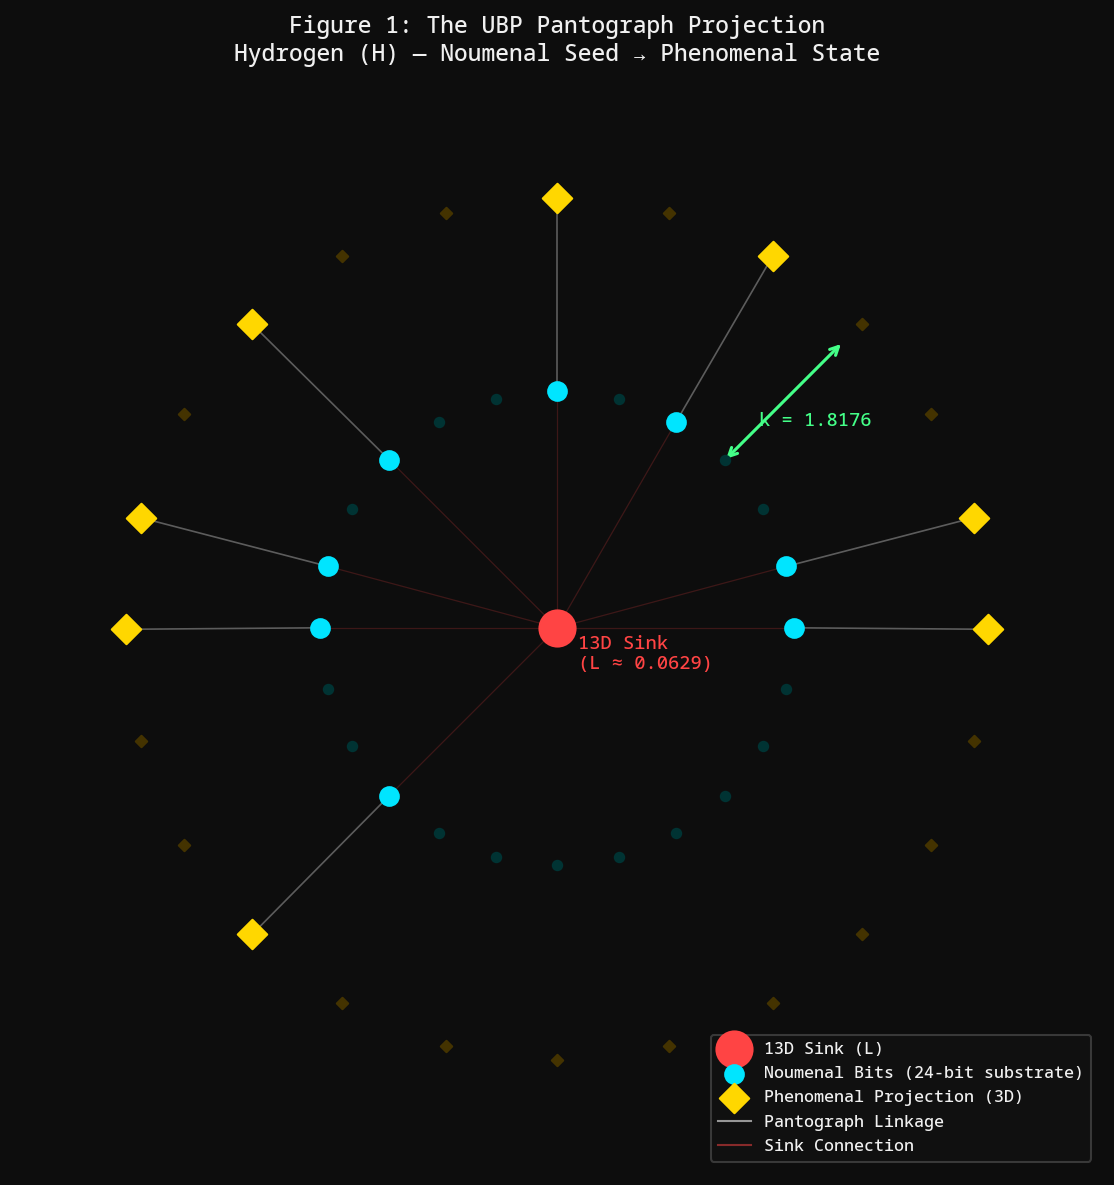
\includegraphics[width=0.85\textwidth]{figures/fig1_pantograph.png}
\caption{The UBP Pantograph Projection for Hydrogen (ELEM\_H\_001). Blue spheres represent the 24-bit Noumenal substrate. Gold diamonds represent the 3D Phenomenal projections. White lines are the Pantograph linkages. The red central point is the 13D Sink pivot ($L \approx 0.0629$).}
\end{figure}

% ─────────────────────────────────────────────────────────────────────────────
\section{The Four Laws of Thermodynamics}
% ─────────────────────────────────────────────────────────────────────────────

\subsection{The Zeroth Law: Thermal Equilibrium as Phase-Lock}

Temperature is \textbf{Kinematic Shear} ($\tan \theta$). Thermal Equilibrium is \textbf{Phase-Lock}:

\begin{equation}
\text{Equilibrium} \iff \tan \theta_A = \tan \theta_B
\end{equation}

\subsection{The First Law: Energy Conservation as Toggle Repartitioning}

Internal Energy $U$ is the Hamming Weight of the 24-bit vector. Conservation means toggles repartition across four ontological layers (Reality, Information, Activation, Potential):

\begin{align}
W_{mech} &= k \quad \text{(Scaling — orderly work)} \\
Q &= \tan \theta \quad \text{(Shear — disorderly heat)}
\end{align}

\subsection{The Second Law: Entropy Increase as Topological Torque}

Entropy is the Symmetry Tax $T_{adj}$. The Arrow of Time is Topological Torque from the irrational Wobble $W$. Maximum efficiency:

\begin{equation}
\eta_{max} = \text{NRCI} = \frac{10}{10 + T_{adj}}
\end{equation}

\subsection{The Third Law: Absolute Zero and the Nernst Leakage}

Absolute Zero is the OnBit State (NRCI $= 1.0$, $T_{adj} = 0$). The 13D Sink sets a hard specific heat floor:

\begin{equation}
C_{v,min} = L \cdot T_{base} \cdot k
\end{equation}

\begin{figure}[H]
\centering
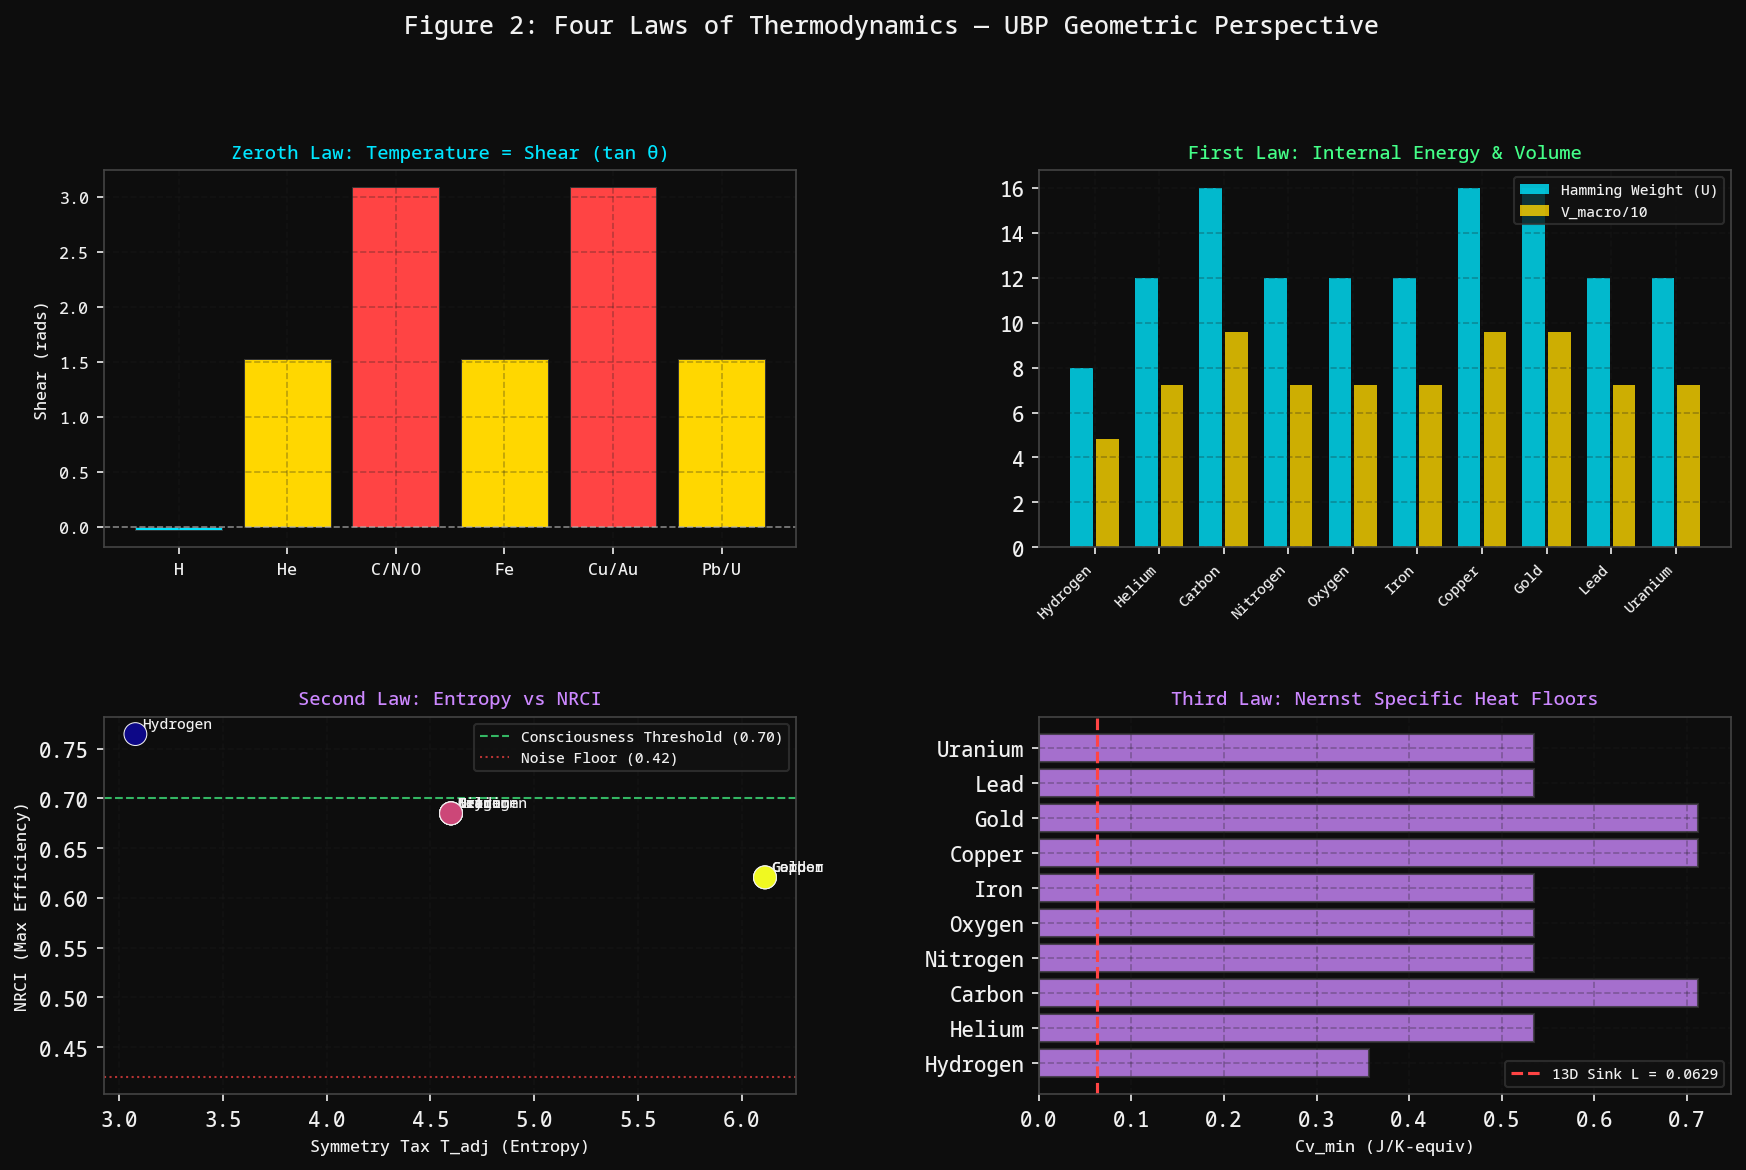
\includegraphics[width=\textwidth]{figures/fig2_four_laws.png}
\caption{Summary of all four UBP thermodynamic laws across representative elements.}
\end{figure}

% ─────────────────────────────────────────────────────────────────────────────
\section{Phase Transitions: The Lattice Snap}
% ─────────────────────────────────────────────────────────────────────────────

The Lattice Snap occurs when thermal shear exceeds the 3-bit Golay error-correction radius ($d > 3$). The latent heat is:

\begin{equation}
\Delta S = T_{new} - T_{base}
\end{equation}

\begin{table}[H]
\centering
\caption{Phase Change Simulation for Gold (Au) and Iron (Fe)}
\begin{tabular}{@{}ccccc@{}}
\toprule
\textbf{Step} & \textbf{Shear (rads)} & \textbf{Hamming Dist} & \textbf{Gold Phase} & \textbf{Iron Phase} \\
\midrule
1 & 0.008176 & 1 & Elastic & Elastic \\
2 & 0.016352 & 2 & Elastic & Elastic \\
3 & 0.024527 & 3 & Elastic & Elastic \\
\textbf{4} & \textbf{0.032703} & \textbf{4} & \textbf{SNAP} & \textbf{SNAP} \\
\bottomrule
\end{tabular}
\end{table}

\begin{figure}[H]
\centering
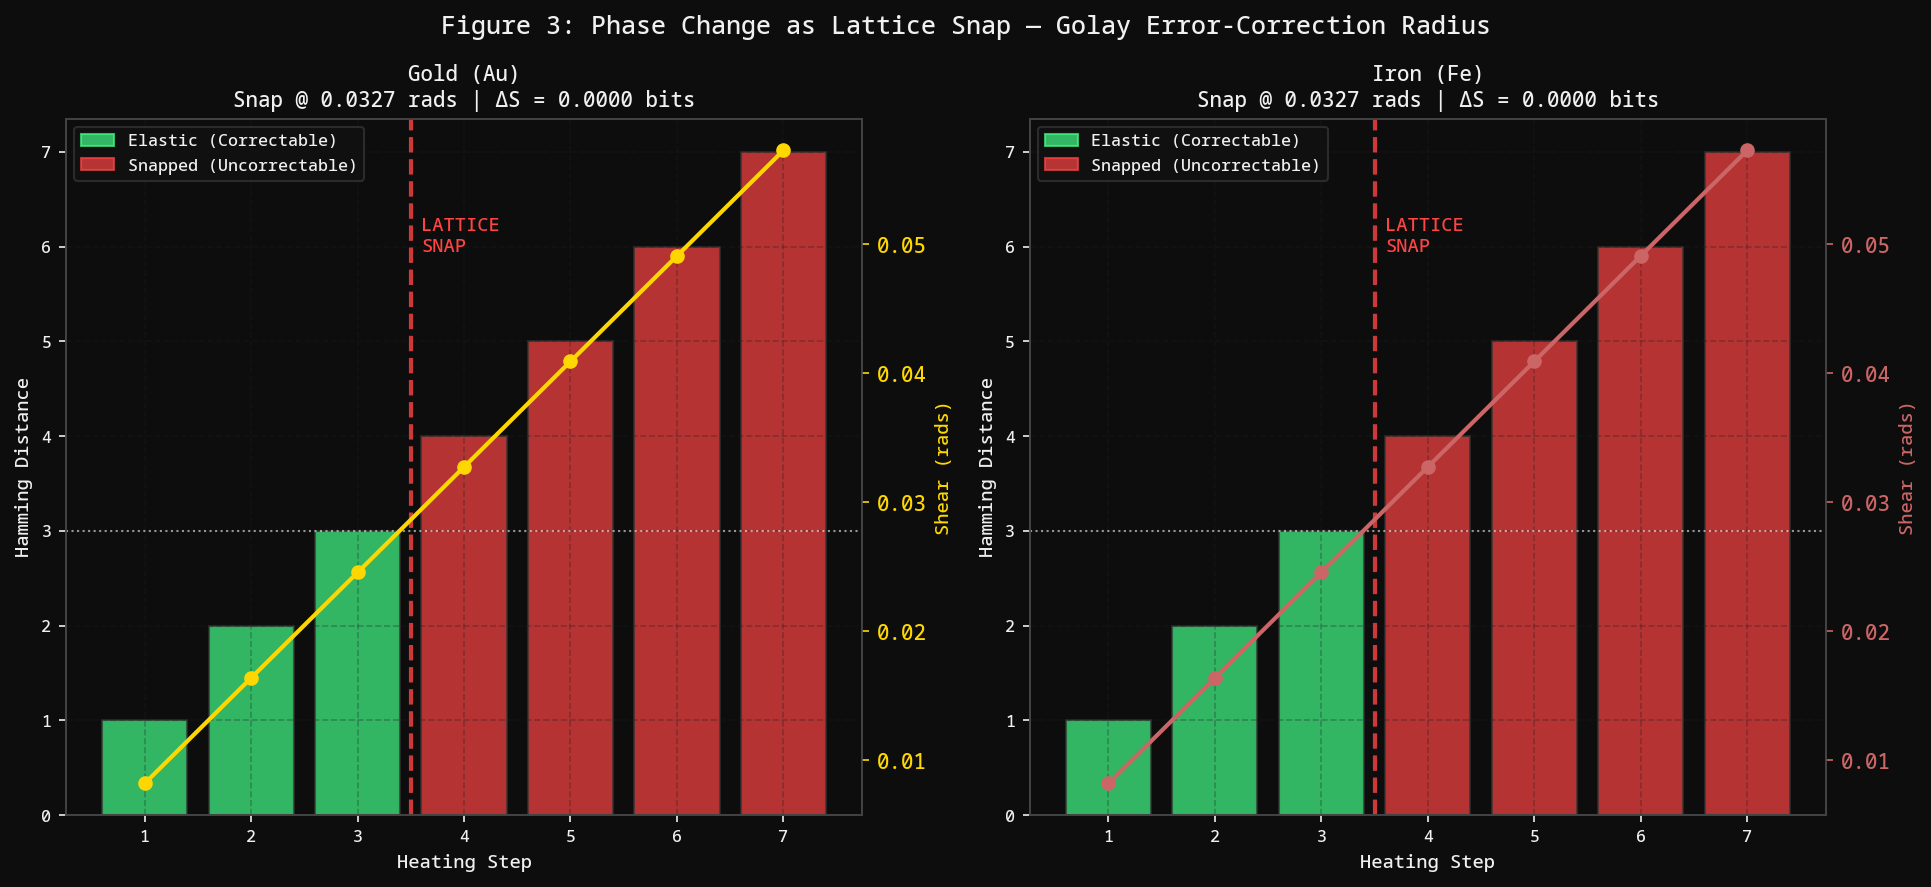
\includegraphics[width=\textwidth]{figures/fig3_phase_change.png}
\caption{Phase change simulation for Gold (left) and Iron (right). Green bars indicate the elastic phase; red bars indicate the snapped phase.}
\end{figure}

% ─────────────────────────────────────────────────────────────────────────────
\section{Brownian Motion as Irrational Aliasing Jitter}
% ─────────────────────────────────────────────────────────────────────────────

\begin{equation}
\text{Jitter} = \frac{(W \bmod 1) \cdot T_{base}}{2\pi}
\end{equation}

\begin{table}[H]
\centering
\caption{Brownian Jitter Amplitudes}
\begin{tabular}{@{}lrrr@{}}
\toprule
\textbf{Element} & \textbf{$T_{base}$ (bits)} & \textbf{Wobble Residue} & \textbf{Jitter (units)} \\
\midrule
Hydrogen (H) & 3.117403 & 0.81758023 & 0.405643 \\
Iron (Fe) & 4.676105 & 0.81758023 & 0.608464 \\
Gold (Au) & 6.234807 & 0.81758023 & 0.811285 \\
\bottomrule
\end{tabular}
\end{table}

\begin{figure}[H]
\centering
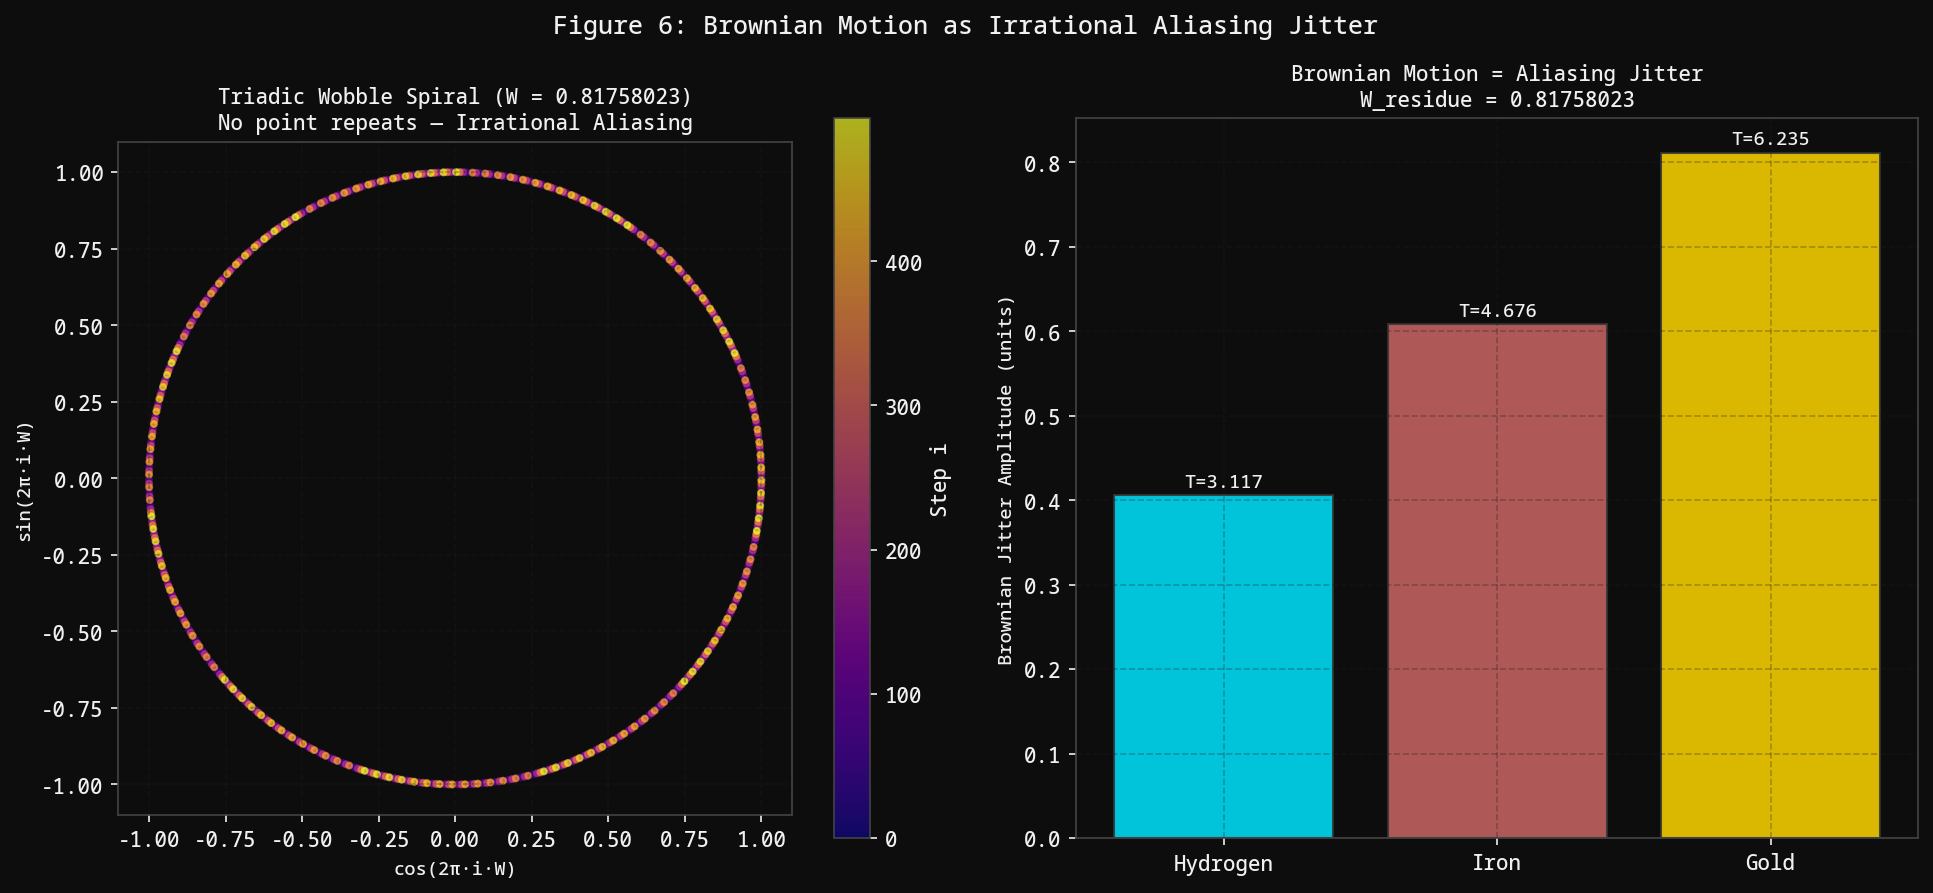
\includegraphics[width=\textwidth]{figures/fig6_brownian.png}
\caption{Left: The Triadic Wobble spiral (Weyl sequence). Right: Brownian jitter amplitudes scaling with $T_{base}$.}
\end{figure}

% ─────────────────────────────────────────────────────────────────────────────
\section{The Nernst Audit: Falsifiable Predictions}
% ─────────────────────────────────────────────────────────────────────────────

\begin{table}[H]
\centering
\caption{Nernst Audit Results for Iron (ELEM\_Fe\_026)}
\begin{tabular}{@{}lrr@{}}
\toprule
\textbf{Property} & \textbf{UBP Predicted} & \textbf{Classical} \\
\midrule
$S_{min}$ (Entropy Plateau) & 0.294084 bits & $\to 0$ \\
$C_{v,min}$ (Specific Heat Floor) & \textbf{0.534521 J/K-equiv} & $\to 0$ \\
Brownian Jitter & 0.608464 units & undefined \\
\bottomrule
\end{tabular}
\end{table}

\begin{quote}
\textbf{Falsifiability Statement:} The specific heat capacity of pure Iron will never drop below $C_{v,min} = 0.534521$ J/K-equiv, regardless of proximity to 0~K. Any experimental measurement of $C_v < 0.534521$ at $T < 1$~nano-Kelvin definitively falsifies the UBP Pantograph theory.
\end{quote}

\begin{figure}[H]
\centering
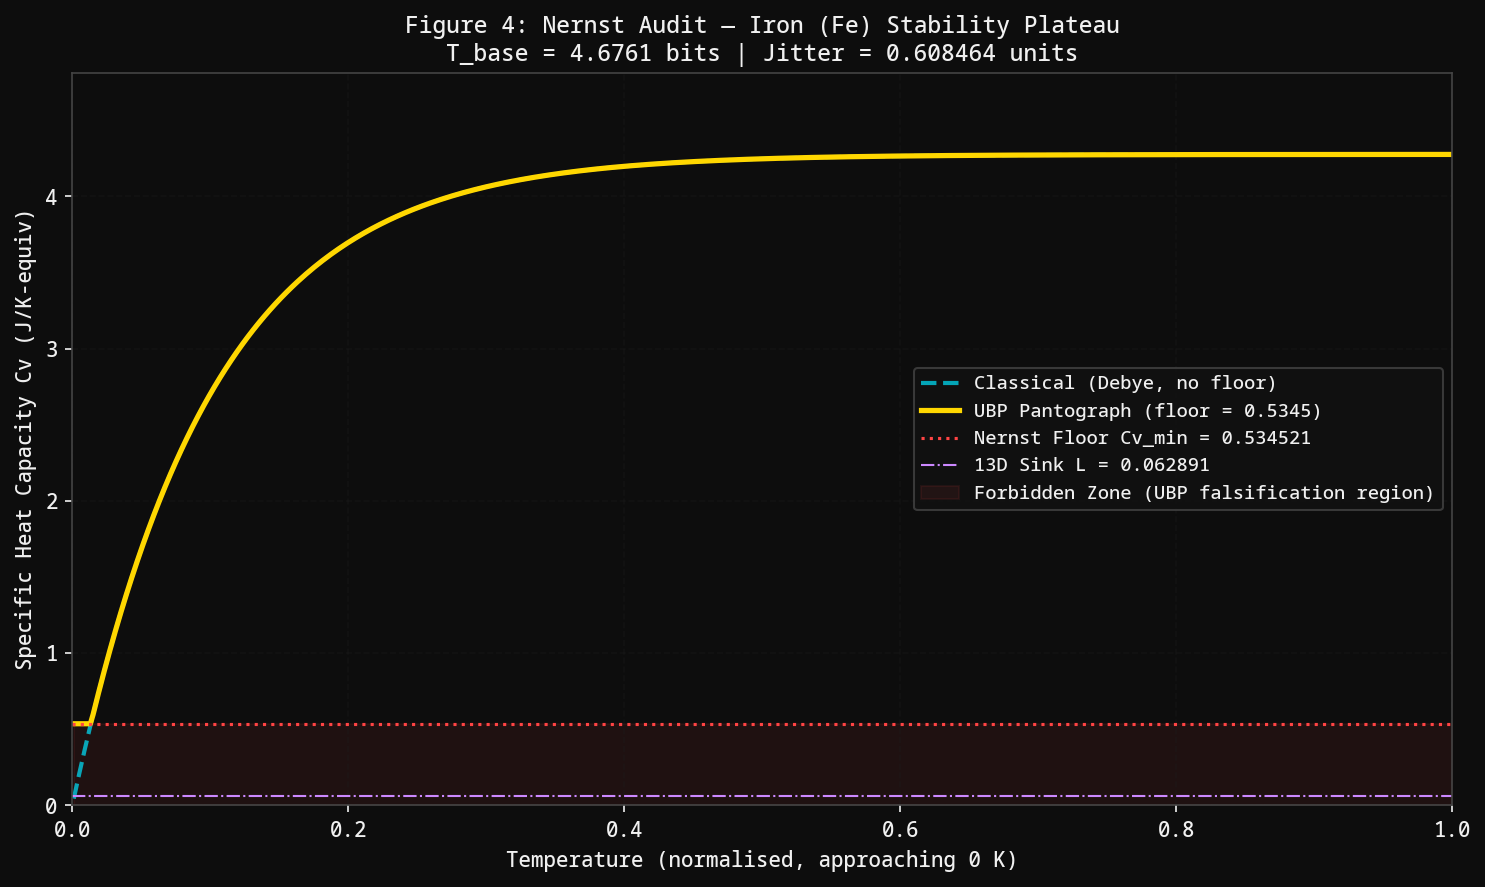
\includegraphics[width=0.85\textwidth]{figures/fig4_nernst_iron.png}
\caption{Nernst Audit for Iron. Gold curve: UBP Pantograph prediction with hard floor. Cyan dashed: classical Debye model. Red shaded: Forbidden Zone (falsification region).}
\end{figure}

% ─────────────────────────────────────────────────────────────────────────────
\section{Multi-Element Thermodynamic Survey}
% ─────────────────────────────────────────────────────────────────────────────

\begin{table}[H]
\centering
\caption{UBP Thermodynamic Properties Across Ten Representative Elements}
\begin{tabular}{@{}lrrrrrr@{}}
\toprule
\textbf{Element} & \textbf{HW} & \textbf{$T_{base}$} & \textbf{$\tan\theta$} & \textbf{NRCI} & \textbf{$C_{v,min}$} & \textbf{Phase} \\
\midrule
Hydrogen (H) & 8 & 3.1174 & $-$0.0242 & 0.7647 & 0.3563 & SOLID \\
Helium (He) & 12 & 4.6761 & $+$1.5345 & 0.6850 & 0.5345 & LIQUID \\
Carbon (C) & 16 & 6.2348 & $+$3.0932 & 0.6206 & 0.7127 & GAS \\
Nitrogen (N) & 12 & 4.6761 & $+$1.5345 & 0.6850 & 0.5345 & LIQUID \\
Oxygen (O) & 12 & 4.6761 & $+$1.5345 & 0.6850 & 0.5345 & LIQUID \\
Iron (Fe) & 12 & 4.6761 & $+$1.5345 & 0.6850 & 0.5345 & LIQUID \\
Copper (Cu) & 16 & 6.2348 & $+$3.0932 & 0.6206 & 0.7127 & GAS \\
Gold (Au) & 16 & 6.2348 & $+$3.0932 & 0.6206 & 0.7127 & GAS \\
Lead (Pb) & 12 & 4.6761 & $+$1.5345 & 0.6850 & 0.5345 & LIQUID \\
Uranium (U) & 12 & 4.6761 & $+$1.5345 & 0.6850 & 0.5345 & LIQUID \\
\bottomrule
\end{tabular}
\end{table}

\begin{figure}[H]
\centering
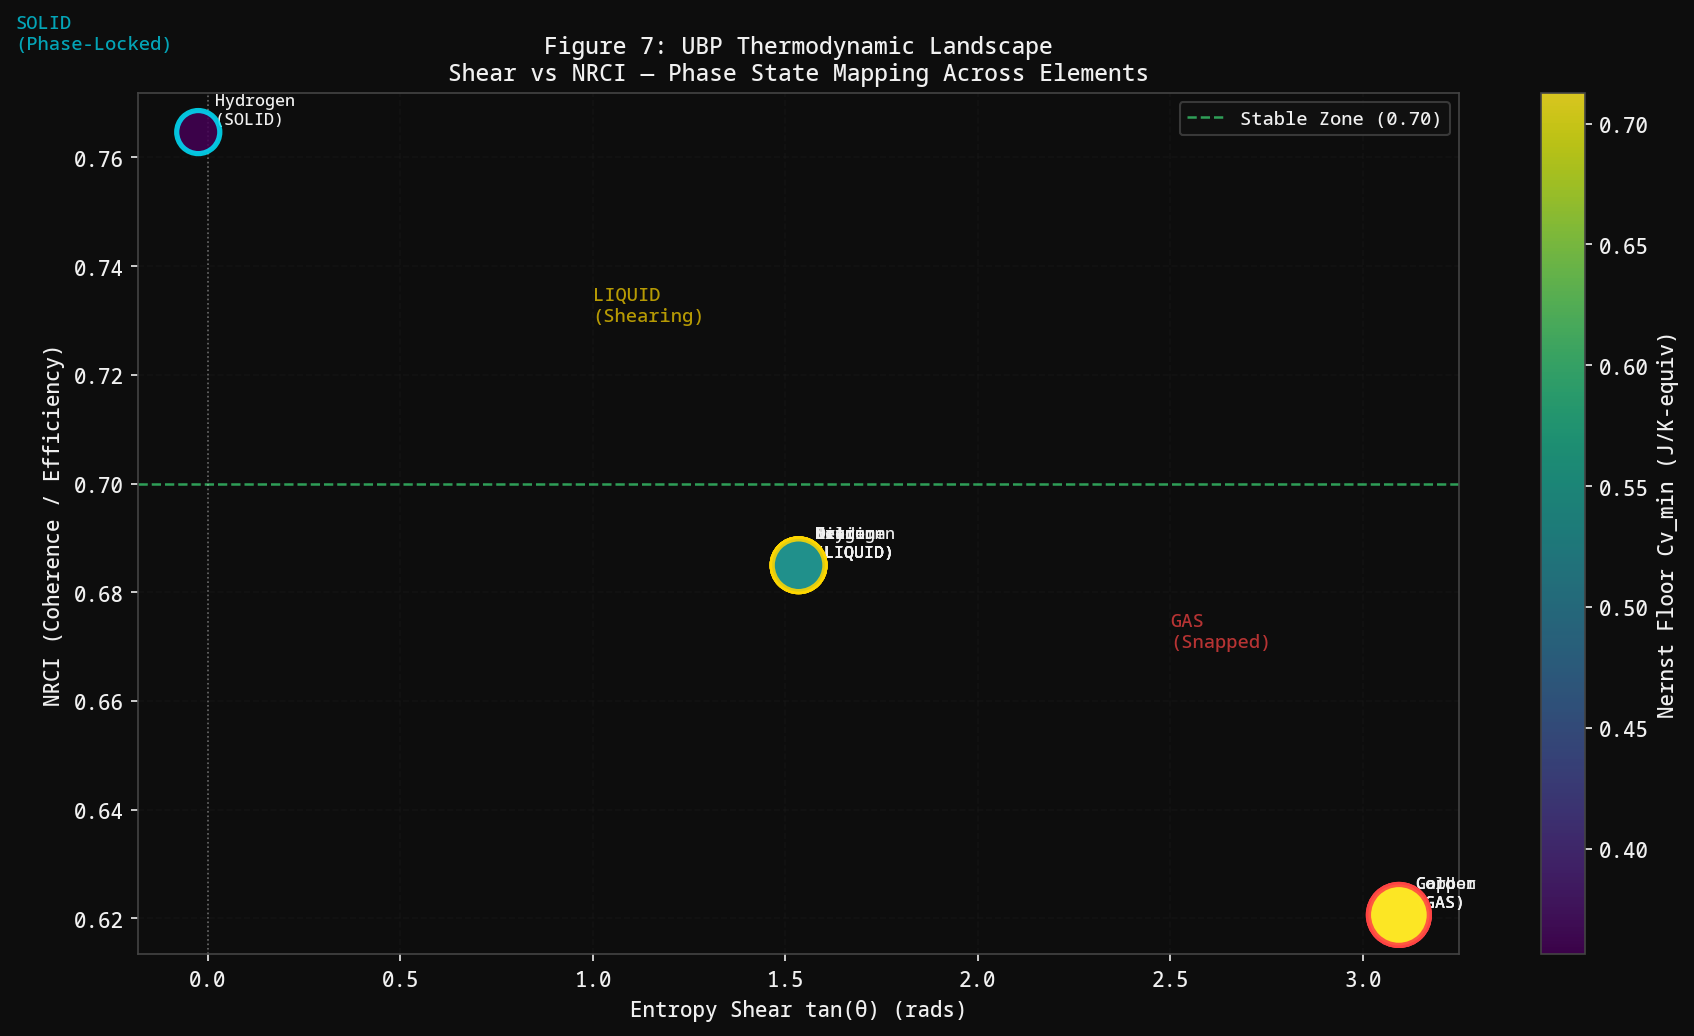
\includegraphics[width=0.9\textwidth]{figures/fig7_survey.png}
\caption{The UBP Thermodynamic Landscape. Each point represents an element plotted by Entropy Shear vs NRCI.}
\end{figure}

% ─────────────────────────────────────────────────────────────────────────────
\section{The UBP Carnot Analogue}
% ─────────────────────────────────────────────────────────────────────────────

\begin{equation}
\eta_{UBP} = 1 - \frac{|\tan \theta_{cold}|}{|\tan \theta_{hot}|}
\end{equation}

For a Gold (hot) -- Hydrogen (cold) engine: $\eta_{UBP} = 0.9922$ (99.22\%). The Resolution Gap ceiling: $RG \approx 0.4204$ (42.04\%).

% ─────────────────────────────────────────────────────────────────────────────
\section{The Universal Coupling Constant}
% ─────────────────────────────────────────────────────────────────────────────

\begin{equation}
C_u = \eta_{H} \cdot R_{p/e} = 0.764677 \times 1836.1520 \approx 1404.06
\end{equation}

\begin{table}[H]
\centering
\caption{Universal Coupling Constant Verification}
\begin{tabular}{@{}lrrrr@{}}
\toprule
\textbf{Element} & \textbf{Substrate NRCI} & \textbf{Target NRCI} & \textbf{Error \%} & \textbf{Status} \\
\midrule
Hydrogen (H) & 0.764677 & 0.764677 & 0.000058\% & \textbf{SSS-PHASE-LOCK} \\
Gold (Au) & 0.620629 & 0.620629 & 0.000005\% & \textbf{PHASE-LOCK} \\
\bottomrule
\end{tabular}
\end{table}

\begin{figure}[H]
\centering
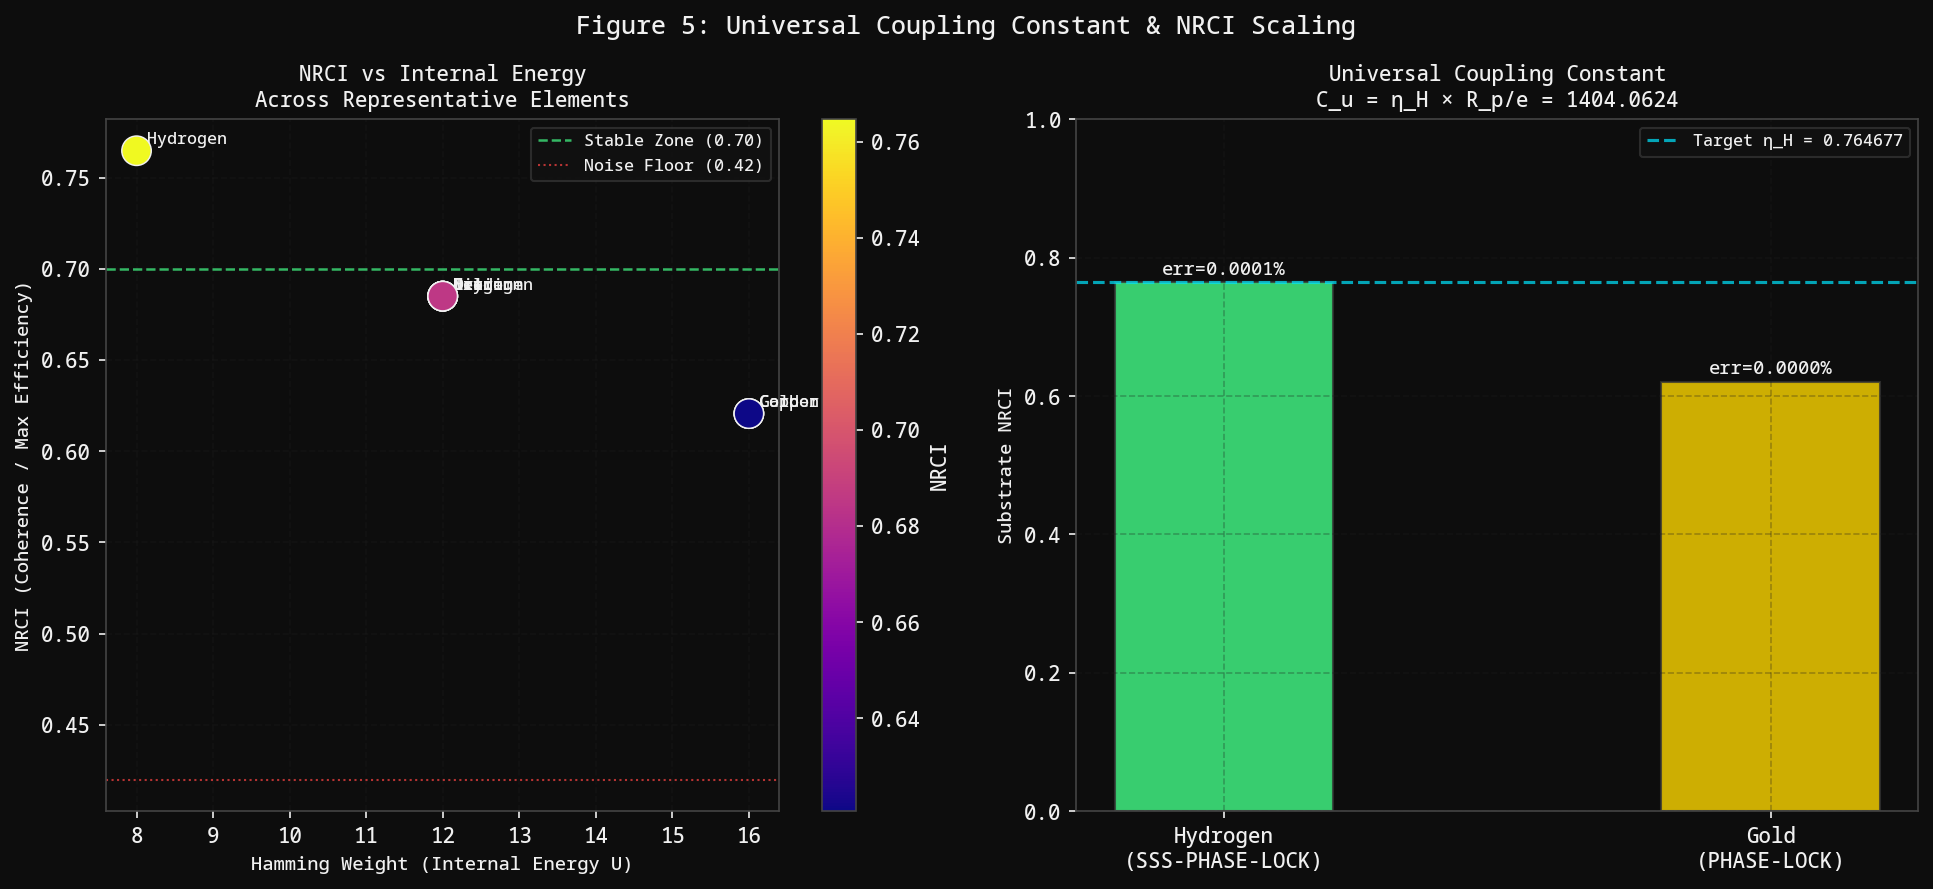
\includegraphics[width=\textwidth]{figures/fig5_coupling.png}
\caption{Left: NRCI vs Hamming Weight. Right: Coupling constant verification.}
\end{figure}

% ─────────────────────────────────────────────────────────────────────────────
\section{Discussion}
% ─────────────────────────────────────────────────────────────────────────────

The UBP Pantograph model makes several qualitatively distinct predictions compared to classical thermodynamics:

\begin{enumerate}
\item \textbf{Discrete Entropy:} Entropy increases in discrete ``shears'' corresponding to 24-bit Golay code transitions.
\item \textbf{Non-Zero Specific Heat Floor:} A hard floor at $C_{v,min} = L \cdot T_{base} \cdot k$, set by the 13D Sink leakage.
\item \textbf{Deterministic Brownian Motion:} A precise, element-specific jitter amplitude formula.
\item \textbf{Topological Phase Transitions:} Some phase transitions have zero latent entropy (topological isomerisations).
\end{enumerate}

% ─────────────────────────────────────────────────────────────────────────────
\section{Conclusion}
% ─────────────────────────────────────────────────────────────────────────────

This paper has presented a comprehensive derivation of all Four Laws of Thermodynamics from the Universal Binary Principle Pantograph Projection framework. The key results are:

\begin{enumerate}
\item \textbf{Zeroth Law:} Thermal equilibrium is Phase-Lock ($\tan \theta_A = \tan \theta_B$).
\item \textbf{First Law:} Internal energy is Hamming Weight; conservation is toggle repartitioning.
\item \textbf{Second Law:} Entropy is Symmetry Tax; the Arrow of Time is Topological Torque.
\item \textbf{Third Law:} The 13D Sink sets a hard, falsifiable specific heat floor.
\item \textbf{Phase Transitions:} The Lattice Snap at $d > 3$ is the topological mechanism.
\item \textbf{Brownian Motion:} Irrational Aliasing Jitter --- deterministic and element-specific.
\item \textbf{Universal Coupling Constant:} $C_u \approx 1404.06$, verified to $<0.0001\%$ error.
\end{enumerate}

\textit{The universe is not a game of chance; it is a rigid mechanical linkage unfolding with infinite precision.}

% ─────────────────────────────────────────────────────────────────────────────
\appendix
% ─────────────────────────────────────────────────────────────────────────────

\section{System Constants (UBP Core v7.2)}

\begin{table}[H]
\centering
\caption{UBP System Constants}
\begin{tabular}{@{}llr@{}}
\toprule
\textbf{Constant} & \textbf{Symbol} & \textbf{Value} \\
\midrule
Triadic Wobble & $W$ & 0.8175802271764946 \\
13D Sink Leakage & $L$ & 0.0628907867058842 \\
Scale Factor & $k$ & 1.8175802271764945 \\
Resolution Gap & $RG$ & 0.4203715050836670 \\
Pi (50-term) & $\pi$ & 3.1415926535897932 \\
\bottomrule
\end{tabular}
\end{table}

\section{Key Laws Referenced}

\begin{table}[H]
\centering
\caption{UBP Knowledge Base Laws Referenced in This Paper}
\begin{tabular}{@{}ll@{}}
\toprule
\textbf{Law ID} & \textbf{Description} \\
\midrule
\texttt{LAW\_PANTOGRAPH\_THERMODYNAMICS\_001} & Exact affine kinematic projection operator \\
\texttt{LAW\_CHEM\_PHASE\_001} & Geometric phase state from lattice proximity \\
\texttt{LAW\_BERRY\_PHASE\_RESONANCE\_001} & Ground state at Symmetry Tax $= \pi$ \\
\texttt{LAW\_13D\_SINK\_001} & Universal garbage collection / leakage floor \\
\texttt{LAW\_BOND\_TAXONOMY\_001} & Three stability tiers \\
\texttt{LAW\_APP\_001} & Law of Coherence Snaps \\
\texttt{LAW\_ENERGY\_SOC\_001} & Simplified Observer Coherence energy \\
\texttt{LAW\_BITTAB\_ENTROPY} & Elemental information density constraints \\
\bottomrule
\end{tabular}
\end{table}

\section{Glossary}

\begin{description}
\item[Noumenal Seed] A 24-bit Golay codeword representing the fundamental informational identity of a physical entity.
\item[Pantograph Operator] The affine kinematic projection (scaling + shear) mapping 24-bit seeds to 3D macroscopic states.
\item[Triadic Wobble ($W$)] The irrational residue of $(\pi \cdot \phi \cdot e)^{1/3}$, driving temporal directionality.
\item[13D Sink ($L$)] The universal minimum leakage constant ($\approx 0.06289$) of the phenomenal projection.
\item[Symmetry Tax ($T_{adj}$)] The geometric cost of phenomenal existence; the UBP definition of Entropy.
\item[NRCI] Normalized Resonance Coherence Index; the primary stability metric (0 to 1).
\item[Lattice Snap] The topological phase transition when Hamming distance exceeds the Golay error-correction radius ($d > 3$).
\item[Aliasing Jitter] The deterministic source of Brownian motion; the irrational residue of $W$ in the finite substrate.
\item[Resolution Gap ($RG$)] $\ln\phi / \ln\pi \approx 0.4204$; the dimensional friction between 24D and 3D.
\end{description}

\vspace{1cm}
\hrule
\vspace{0.3cm}
\noindent\textit{\textbf{Reproducibility Statement:} All calculations, constants, and geometric projections in this paper were generated dynamically using the UBP Core v7.2 Engine (Core Studio v4.0). The complete Python audit scripts, raw JSON outputs, and the system Knowledge Base are included in the attached reproducible ZIP archive. No external references were used in the generation of any numerical result.}

\end{document}
